\documentclass{article}

\usepackage{fancyhdr} % Required for custom headers
\usepackage{lastpage} % Required to determine the last page for the footer
\usepackage{extramarks} % Required for headers and footers
\usepackage[usenames,dvipsnames]{color} % Required for custom colors
\usepackage{graphicx} % Required to insert images
\usepackage{listings} % Required for insertion of code
\usepackage{courier} % Required for the courier font
\usepackage{caption}
\usepackage{multirow, float}
\usepackage{subcaption}
\usepackage{graphicx}


\renewcommand{\_}{\char`_}
\renewcommand{\tt}{\lstinline}

% Margins
\topmargin=-0.45in
\evensidemargin=0in
\oddsidemargin=0in
\textwidth=6.5in
\textheight=9.0in
\headsep=0.25in

\linespread{1.1} % Line spacing


% Set up the header and footer
\pagestyle{fancy}
\lhead{Group 24} % Top left header
\chead{Corsair} % Top center head
\rhead{\firstxmark} % Top right header
\lfoot{\lastxmark} % Bottom left footer
\rfoot{Page\ \thepage\ of\ \protect\pageref{LastPage}} % Bottom right footer
\renewcommand\headrulewidth{0.4pt} % Size of the header rule
\renewcommand\footrulewidth{0.4pt} % Size of the footer rule

\setlength\parindent{0pt} % Removes all indentation from paragraphs

%----------------------------------------------------------------------------------------
%	TITLE PAGE
%----------------------------------------------------------------------------------------

\title{
\vspace{2in}
\textmd{\textbf{Project Management}}\\
\normalsize\vspace{0.1in}\small{Due\ on\ Monday,\ June\ 6,\ 2016}\\
\vspace{0.1in}\large{\textbf{WebApps Group 24: Corsair}}
\vspace{3in}
}

\author{Mery Noa Bendahan \\ Ignacio Navarro \\ Dan Slocombe \\ Tom Griggs \\ Jaime Rodriguez}
\date{}

%----------------------------------------------------------------------------------------

\begin{document}

\section{Project Management}
We have chosen to use Agile methodologies for project management, so we have focused on the following: Continuous improvement and delivering quality product. As a project management tool we have used Agile Planner- an app for iterative development teams: Here we illustrate the state of our board at different stages of the week for the second iteration.
This tool allowed us to create cards with tasks and move them around from To-do to delivered. In a single card we could add comments, discussions, tags, developers, contributors as well as a detailed description of what was needed.

\begin{figure}[ht] 
  \label{ fig7} 
  \begin{minipage}[b]{0.5\linewidth}
    \centering
    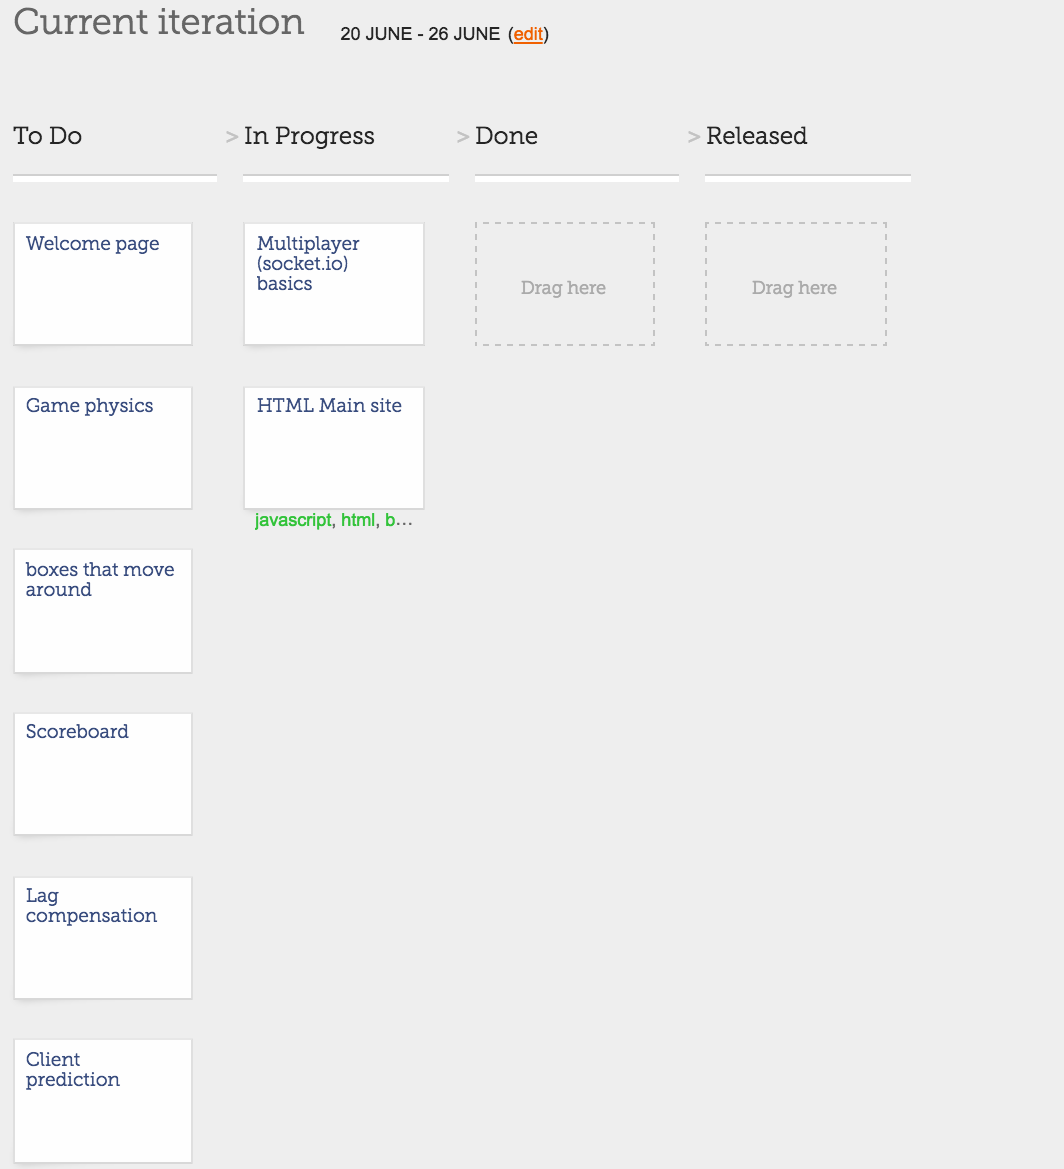
\includegraphics[width=.8\linewidth]{beginning} 
    \caption{Board at the beginning of the iteration} 
    \vspace{4ex}
  \end{minipage}%%
  \begin{minipage}[b]{0.5\linewidth}
    \centering
    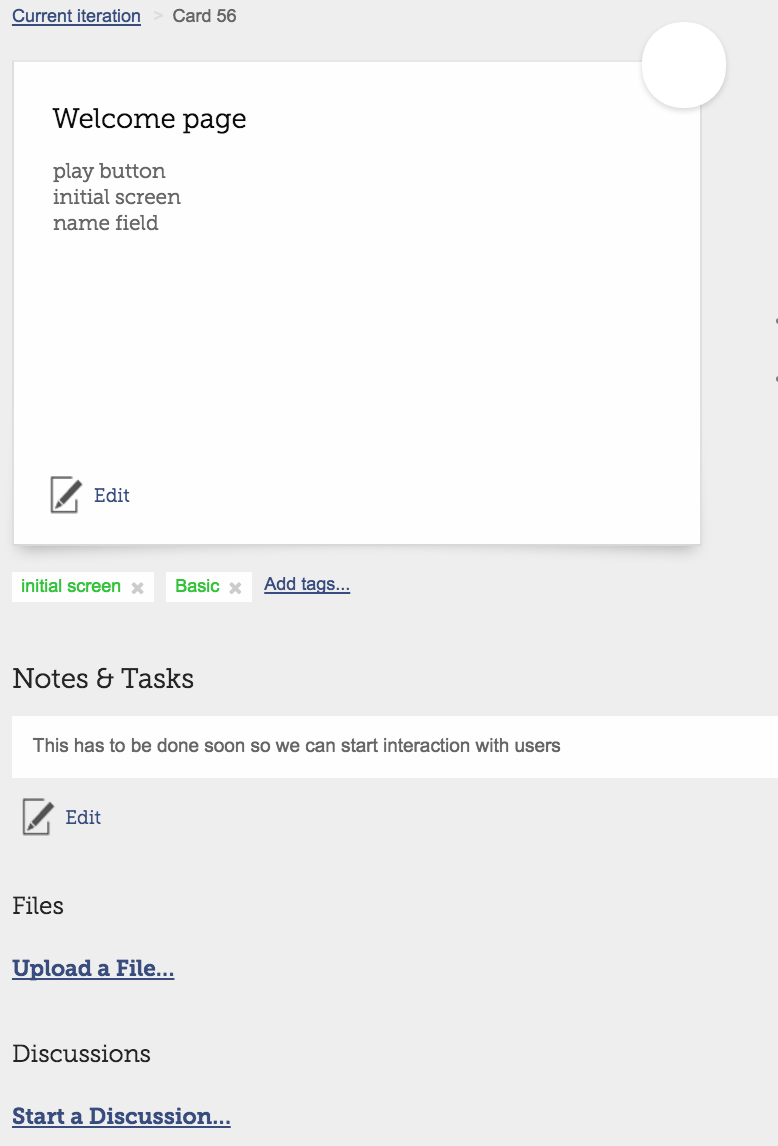
\includegraphics[width=.6\linewidth]{card} 
    \caption{A single card and its content} 
    \vspace{4ex}
  \end{minipage} 
  \begin{minipage}[b]{0.5\linewidth}
    \centering
    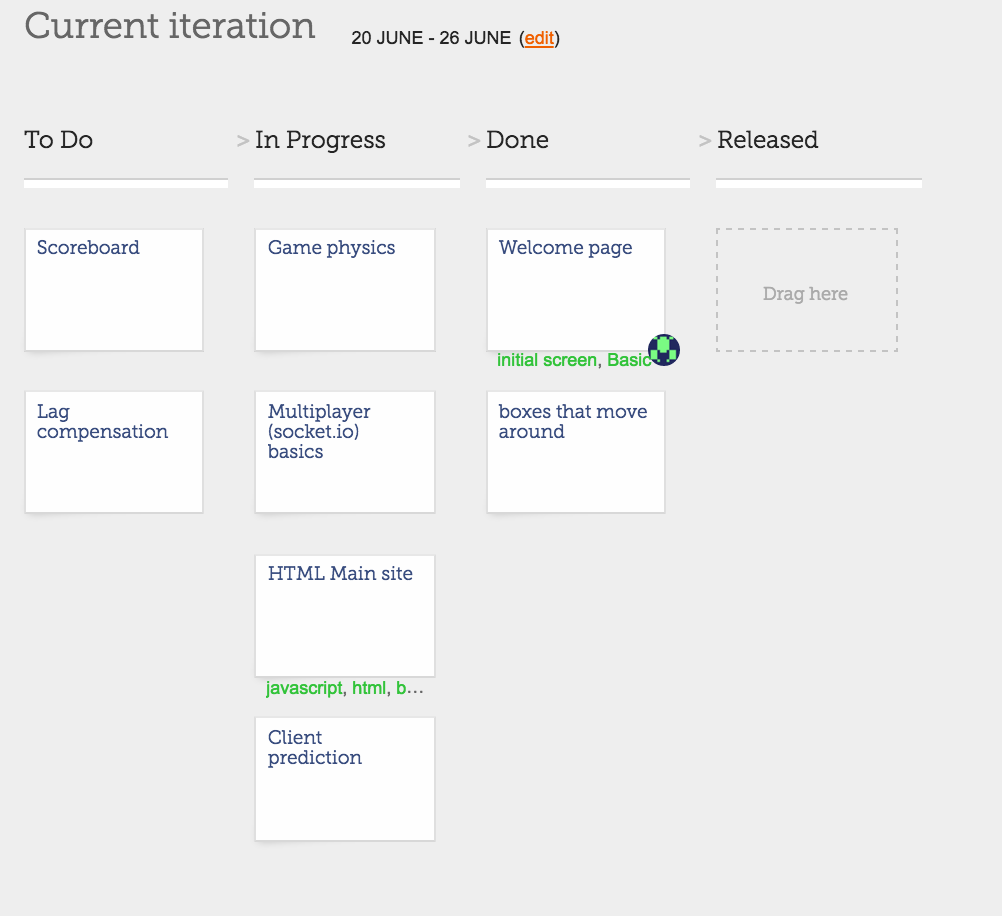
\includegraphics[width=.85\linewidth]{middle} 
    \caption{Board at the middle of the iteration} 
    \vspace{4ex}
  \end{minipage}%% 
  \begin{minipage}[b]{0.5\linewidth}
    \centering
    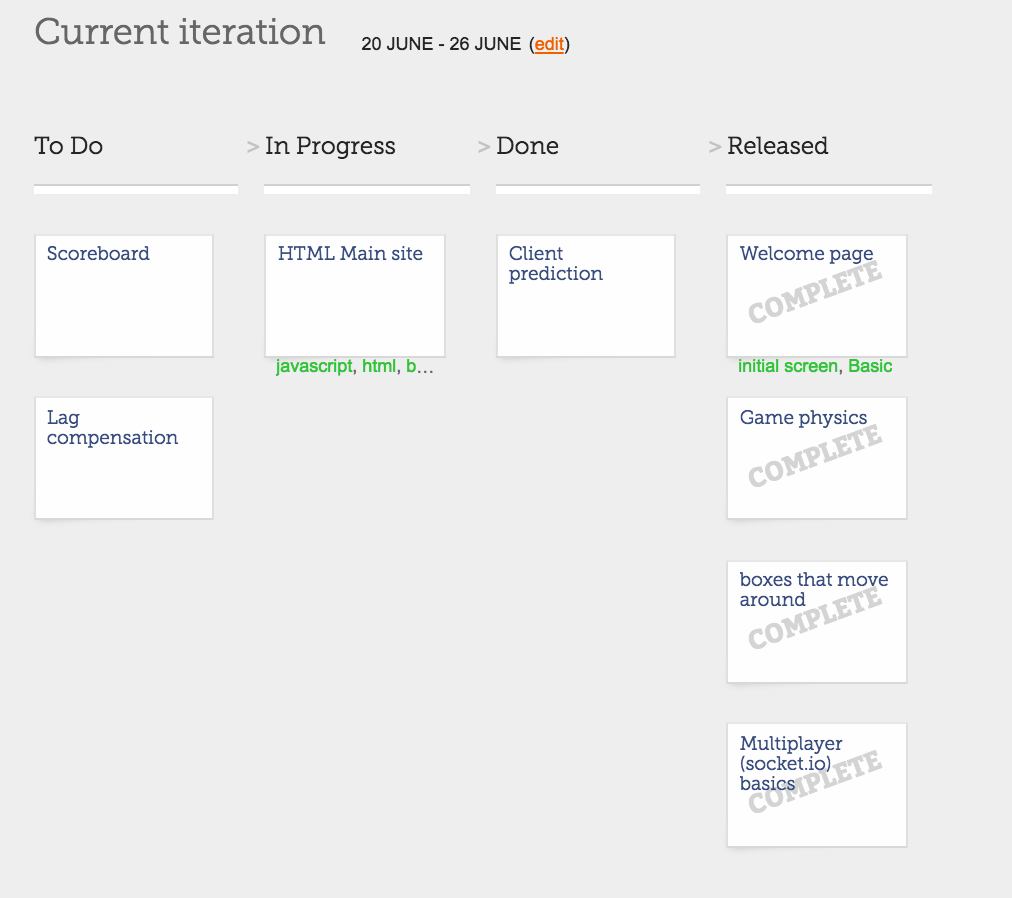
\includegraphics[width=.85\linewidth]{end} 
    \caption{Board at the end of the iteration} 
    \vspace{4ex}
  \end{minipage} 
\end{figure}

\end{document}
